
%% DAN CHECKING INTERPRETATIONS OF G' and G'' and length scales etc 

%1)	Check legends in all G’/G’’ plots.

%2)	Fig 2, frequency units shown as rad/S instead of rad/s

%3)	Not sure about the 1/alpha exponent for G’ and G’’ - this should scale with alpha not 1/alpha but lets check …..do we have the MSD(tau) curve for the GP. 



%got to line 204


\documentclass[%
 aip,
% jmp,
% bmf,
% sd,
% rsi,
 amsmath,amssymb,
%preprint,
reprint, onecolumn %%%%% Comment onecolumn to override one column format %%%%%%%
%author-year,%
%author-numerical,%
% Conference Proceedings
]{revtex4-1}

\usepackage{graphicx}% Include figure files
\usepackage{dcolumn}% Align table columns on decimal point
\usepackage{bm}% bold math
%\usepackage[mathlines]{lineno}% Enable numbering of text and display math
%\linenumbers\relax % Commence numbering lines

\usepackage[utf8]{inputenc}
\usepackage[T1]{fontenc}
\usepackage{mathptmx}
\usepackage{etoolbox}
\usepackage{gensymb}
\usepackage{xcolor}
%% Apr 2021: AIP requests that the corresponding 
%% email to be moved after the affiliations
\makeatletter
\def\@email#1#2{%
 \endgroup
 \patchcmd{\titleblock@produce}
  {\frontmatter@RRAPformat}
  {\frontmatter@RRAPformat{\produce@RRAP{*#1\href{mailto:#2}{#2}}}\frontmatter@RRAPformat}
  {}{}
}%
\makeatother

\begin{document}

\preprint{AIP/123-QED}

% Force line breaks with \\
\title{Modelling of Microrheology on Idealised Percolation Gelling Systems}
% Force line breaks with \\
\author{D. W. James}
\author{D. J. Curtis}%
\author{M. R. Brown*}
    \email{m.r.brown@swansea.ac.uk}
\affiliation{Complex Fluids Research Group, Faculty of Science and Engineering, Swansea University, Swansea, SA1c 8EN
}%
%


\begin{abstract}
Microrheology experiments study the rheological properties of viscoelastic materials by tracking the diffusion of embedded microscale particles. The elastic and viscous moduli $G^{'}(\omega)$ and $G^{''}(\omega)$ can be extracted via the Generalised Stokes Einstein relations (GSER) applied to the ensemble averaged mean square displacement (MSD). When such techniques are applied to heterogeneous systems with microstructural length-scales on the order of the probe diameters, a significant discrepancy occurs between micro and bulk rheological results. In this work, we use percolation lattices and random walks as an idealised model of microrheology experiments on heterogeneous gelling systems. Three different regimes of MSD and corresponding $G^{'}(\omega)$ and $G^{''}(\omega)$ curve features are identified and typical characteristics of a sol-gel transition, including independent power laws in $G^{'}(\omega)$ and $G^{''}(\omega)$, are demonstrated. We establish that frequency independence in the loss tangent occurs at the percolation threshold of unoccupied sites ($p'_c$), not at the percolation threshold of occupied sites ($p_c$) that represents the true gel point. This definitively explains why microrheology predicts a later gel point than bulk rheology in 3D heterogeneous systems. We develop a time-dependent percolation model that maps percolation probability to experimental time, enabling quantitative prediction of the lag between true and apparent gel points as $\Delta t = \frac{1}{k}\ln\left(\frac{p_\infty-p'_c}{p_\infty-p_c}\right)$. Additionally, features of MSD curves usually attributed to cage hopping and relaxation of networks are shown to arise from the self-similar nature of the network and its embedding space, demonstrating that structural features alone can generate complex MSD behaviours without dynamic mechanisms.
\end{abstract}

\maketitle


\section{Introduction}

Microrheology can be used to determine the rheological properties of viscoelastic materials by tracking the displacement of embedded microscale probe particles over time. Displacements can be driven by an applied force \cite{Bausch1999,Gardel2005,Cappella2005} or by thermal fluctuations \cite{Oppong2006}, referred to as active or passive microrheology, respectively. Advantages of microrheology over traditional bulk rheological techniques include the ability to investigate the local dynamics and structure of a material on smaller length-scales and extension of the experimental frequency range to lower frequencies \cite{Larsen2008,Moschakis2013}.

Microrheological techniques have evolved significantly in recent years, with substantial improvements in both experimental methods and data analysis. For example, advanced particle tracking algorithms now incorporate machine learning approaches that significantly improve accuracy in heterogeneous media \cite{Koens2018}. Active microrheological techniques employing optical tweezers have been refined to address limitations in heterogeneous systems \cite{Tassieri2019}. These advancements have enabled more reliable measurements in complex biological materials where microstructural heterogeneity previously posed significant challenges. Despite these technological improvements, the fundamental interpretation of MSD data in heterogeneous systems continues to present theoretical challenges \cite{Waigh2022}, particularly regarding the accurate determination of the gel point, which this work aims to address.
Many viscoelastic materials undergo a sol-gel transition, where the connectivity of a microstructural network within the material increases until it is able support stress, effectively transitioning the bulk sample from a viscoelastic liquid to a viscoelastic solid. The point of transition is referred to as the gel-point (GP). The network structure of a material at the GP is important for a wide range of applications and industries including health care diagnostics \cite{Evans2010a,Evans2008,Evans2010b}, stability in food systems \cite{Moschakis2013}, stability of emulsions \cite{Oliveira2010}, semi-conductor crystal growth \cite{Spanhel1991} and colloidal systems \cite{Coniglio2004}. An important sol-gel transition for health care applications occurs during the process of blood coagulation \cite{Curtis2014,Badiei2015,Hawkins2010}. The microstructure of the incipient clot (i.e., the clot as it exists at the GP) is an indicator of healthy haemostasis \cite{Collet2000,Collet2005,Weisel2007}. Furthermore, the incipient clot acts as a template for further clot evolution \cite{Curtis2013}.

The sol-gel transition is a percolation process, where small solid fractal clusters form and aggregate to eventually establish an incipient sample spanning cluster (in addition to smaller finite clusters, with a range of sizes, which are not attached to the sample spanning cluster). Between lower and upper limits of the fractal scaling, the mass of the network scales self-similarly as $m\sim l^{d_{f}}$(where, $m$ , $l$ and $d_{f}$ denote mass, Euclidean distance and fractal dimension, respectively). The upper limit of self-similar scaling provides a correlation length $\xi$ which, pre-GP, is a measure of the average span of clusters and increases as the system evolves towards the GP due to cluster growth. At the GP, $\xi$ diverges and the incipient sample-spanning cluster exhibits a self-similar scaling over all length-scales \cite{Curtis2013}. Smaller clusters are located within pore spaces embedded within the sample-spanning cluster. Post-GP $\xi$ is finite and represents the span of the largest pores in the system \cite{Ben-Avraham2000}.

According to the theory of Winter \& Chambon \cite{Chambon1987}, at the GP the viscoelastic storage and loss moduli, scale as power laws in frequency,  $G^{'}(\omega)\ {\sim\ G}^{''}(\omega)\ \sim\omega^{n}$, where $n$ is the stress relaxation exponent \cite{Larsen2008}.
Equivalently, the GP can be identified by frequency independence of the loss tangent $\tan\delta\left( = G^{''}/G^{'} \right)$ where $\delta$
represents the phase angle between the applied oscillatory perturbation (stress or strain) and the response of the material to that perturbation \cite{Chambon1987}. At the GP $\delta = n\pi/2$ where lower $\delta$ indicates higher network branching \cite{Muthukumar1989}. For freely jointed polymer networks, the fractal dimension of the incipient network can be obtained from $\delta$ at the GP using Muthukumar's relation, allowing structural characterisation of the network using rheological data \cite{Muthukumar1989,Muthukumar1985}.

In microrheology experiments $G^{'}(\omega)$ and $G^{''}(\omega)$ can be obtained by applying the generalised Stokes-Einstein relation (GSER) to the time-averaged mean square displacement (MSD) of probe particles\cite{Mason1995,Mason2000}. The MSD is given as MSD $\equiv \left\langle \mathrm{\Delta}r^{2}(\tau) \right\rangle = \ \left\langle \left\lbrack \mathbf{r}(\tau + t) - \mathbf{r}(t) \right\rbrack^{2} \right\rangle$, where $\mathbf{r}$ is the displacement vector and $\left\langle \ldots \right\rangle$ indicates an average over all probe particle displacements and over the lag-time $\tau$ \cite{Moschakis2013}. In a purely viscous material, the probe particles will undergo regular diffusion and the MSD will be of the form

\begin{equation}
\left\langle \mathrm{\Delta}r^{2}(\tau) \right\rangle = 2dD\tau
\end{equation}
where $d$ is the embedding dimension and $D$ is the diffusion coefficient. For a purely elastic material, the maximum displacement of the probe particles is bounded and the MSD is independent of $\tau$ \cite{Moschakis2013}. For intermediate viscoelastic materials pre-GP, anomalous diffusion is often exhibited and the MSD power-law relation as a function of $\tau$ is expressed as:

\begin{equation}
\left\langle r^{2}(\tau) \right\rangle \sim \ \tau^{\alpha}
\end{equation}

where $\alpha$ is the anomalous diffusion exponent \cite{Moschakis2013}. Sub-diffusive anomalous diffusion is indicated by {$ \tau$ independence} when $\alpha< 1$. At the GP the MSD is expected to obey equation 2 for all $\tau$ due to the divergence of $\xi$ \cite{Moschakis2013}.

The formulation of the GSER assumes that the embedding material appears homogeneous on the length-scale of the probe particles \cite{Mason1995,Mason2000,Oppong2006}. Excellent agreement for measured $G^{'}(\omega)$
$G^{''}(\omega)$ and GP has been demonstrated between microrheology and bulk shear rheometry experiments adhering to this condition \cite{Larsen2008,Dasgupta2002,Dasgupta2005}. However, there is little correspondence between $G^{'}(\omega)$ and $G^{''}(\omega)$ obtained by microrheology and bulk rheology experiments when the material appears heterogeneous on the length-scale of probe particles, resulting in a significant disparity between the predicted GP and that measured through microrheology experiments \cite{Rich2011,Oppong2006}. For heterogeneous systems, the probe particles predominately move within the fluid filled pores embedded within the elastic network. This condition results in the diffusion being impeded by discrete collisions with the gel network, as opposed to the continuous restoration force imposed by an elastic network \cite{Moschakis2013,deBruyn2013}. Despite awareness of this discrepancy, the fundamental mechanisms underlying it remain incompletely understood.

In this work, we utilise percolation lattices as an idealised model system to investigate microrheology in heterogeneous gelling materials. This approach offers several key advantages:
\begin{enumerate}
    \item We isolate the structural effects on probe dynamics by modelling random walks on unoccupied sites of percolation lattices, providing a controlled environment where interactions with occupied sites (representing the gel structure) are the only source of probe impediment.
    \item We systematically analyse how the MSD curves evolve throughout the percolation process, identifying characteristic regimes and their underlying structural causes.
    \item We establish a quantitative relationship between percolation parameters and time-dependent gelation processes, creating a bridge between our computational model and experimental rheology.
    \item We develop a transformation framework that maps percolation probability $p$ to experimental time $t$ using the relationship $p(t) = p_\infty(1-e^{-kt})$, enabling the direct translation of our percolation-based findings to time-dependent rheological measurements.
    \item We provide a mechanistic explanation for the observed discrepancy between gel points determined by bulk rheology and microrheology in heterogeneous systems.
    \item We demonstrate that structural features alone can generate MSD behaviours typically attributed to dynamic processes such as cage-hopping and network relaxation.
\end{enumerate}
Through this approach, we aim to develop a comprehensive theoretical framework for interpreting microrheological data in complex systems with significant heterogeneity, addressing a critical gap in our understanding of how structural features influence rheological measurements and enabling more accurate determination of the gel point in heterogeneous materials.

\section{Methods}
\subsection{Gelling lattice system}

In a percolation lattice system, each site in the lattice is occupied with a probability $p$. For $p$ below a critical value $p_{c}$, randomly occupied sites form isolated clusters. These clusters are fractal in nature and the upper limit on their size is dependent on the correlation length of the lattice $\xi_{latt}$. As $p \rightarrow p_{c}$ the correlation length diverges and, for a theoretical infinite lattice, when $p\sim p_{c}$, an infinite percolation cluster forms, containing pores on all length-scales. For finite lattices, $p_{c}$ represents the most probable value of $p$ at which percolation occurs \cite{Stauffer1992,Stauffer2007}. For $p > p_{c}$, as with the sol-gel system post-GP, the correlation length decreases with $p$.

Recent developments in percolation theory have extended our understanding to multi-component systems with distinct types of nodes \cite{Grimaldi2019}, providing additional theoretical frameworks for analysing the relationship between occupied and unoccupied site percolation. These advancements are particularly relevant for understanding real heterogeneous systems where the basic network and void spaces have fundamentally different geometries. Additionally, scale-dependent dynamics in heterogeneous soft materials have been empirically confirmed through advanced microrheology experiments \cite{Lindner2021}, validating many theoretical predictions about length-scale dependent probe dynamics that are central to our modelling approach.

Percolation lattices can therefore be viewed as an idealised model of a sol-gel transition, where percolation represents the GP. Diffusion processes, such as those occurring in passive microrheology experiments, can be understood as random walks at the continuum limit \cite{deBruyn2013}. Random walk simulations are routinely performed on percolation lattices, on either the occupied \cite{Ben-Avraham2000,Havlin1983} or unoccupied \cite{Saxton1994,Saxton1993,Saxton1997} lattice sites. Typically, in these simulations, a walker will attempt to move into a randomly chosen neighbouring lattice site, remaining in its current site if the neighbouring site is occupied.

Their MSDs exhibit anomalous and regular diffusion behaviours, when $\sqrt{MSD} \ll \xi_{latt}$ and $\sqrt{MSD} \gg \xi_{latt}$, respectively \cite{Stauffer1992,Stauffer2007}. Considering percolation lattices as an idealised model of a gelling system, it follows that random walk simulations on the unoccupied sites of percolation lattices represent an idealised model of microrheology experiments performed on a heterogeneous system \cite{deBruyn2013}.

Randomly occupied sets of 3D lattices were generated for a range of values of $p$, assuming a micro-canonical ensemble, thus eliminating fluctuations \cite{Newman2000,Newman2001}. For each set of lattices an initial lattice was generated with $p = 0.01$. Further lattices were generated sequentially, incrementing the value of $p$ by $p_{inc}=0.01$ from the previous lattice in the system. Successive lattices retain the occupied sites from the previous lattice and further sites for occupation are selected randomly from the unoccupied sites, satisfying $p_{i + 1} = \ p_{i} +$ $p_{inc}$ (where $i$ is the index of the sequence). Lattice sets were generated in this way to mimic the sol-gel transition and the templating function of the incipient sample-spanning gel microstructure \cite{Curtis2013}. Herein, a set of sequentially generated lattices are referred to as the gelling lattice system. Ten distinct gelling lattice systems were realised with lattice dimensions of $100\times100\times100$.

This computational approach, while well-established, represents one point in a spectrum of increasingly sophisticated simulation methods. Modern computational approaches to random walk simulations have expanded beyond these simple lattice models to include more complex environments and analysis techniques. For instance, recent work by Sentjabrskaja et al. \cite{Sentjabrskaja2019} has examined anomalous dynamics of intruders in crowded environments with mobile obstacles, providing a more complex but realistic extension of the static obstacle model presented here. Additionally, the analysis of MSD curves has been revolutionised by machine learning approaches that can identify subtle features in particle trajectories previously inaccessible to traditional analytical methods \cite{Li2020}. While we employ classical percolation theory and random walk dynamics in this work, for their clarity and fundamental nature, these newer computational advances offer promising directions for future refinements of our model, particularly for systems where obstacles have their own dynamics.

\subsection{Random Walks}

Random walks were performed on unoccupied lattice sites, representing the fluid-filled spaces within the gel structure. The blind ant step model of de Gennes \cite{Stauffer1992} was employed in all random walk simulations. At each time step the probe attempted to move into a stochastically chosen adjacent site within its von Neumann neighbourhood (i.e., periodic boundary conditions) \cite{Margolus1987}. If the site was occupied the probe remained in its current location. Each simulation had $10^5$ time steps. The MSD was calculated by averaging over $10^{3}$ distinct walks for each lattice considered. Additionally, MSDs were averaged over lag-time, $\tau$ \cite{Moschakis2013}. For each random walk the first $10^3$ pairs of displacements separated by lag-time $\tau$ were used for averaging. For random walks on fractal structures the MSD curves for lag-time averaged and non-lag-time averaged instances are equivalent \cite{Havlin1983}. Lag-time averaging acts only to reduce the noisiness inherent to diffusion processes. The simulation routine was written in C++.

\subsection{Calculation of $G'(\omega)$ and $G''(\omega)$}

For a typical microrheology experiment the time and spatial resolution of imaging equipment presents a lower limit on measurable lag-time $\tau$ and displacement $\mathbf{r}$, respectively (though techniques are available for sub-pixel resolution measurements \cite{Chenouard2014,Rodriguez2016}). We refer to the equivalent quantities in random walk simulations as $\tau^{*}$ and $\mathbf{r}^{*}$, which represent the number of attempted steps by a walker and the linear dimension of a lattice site respectively \cite{Gefen1983,Saxton1994}. These quantities have dimensionless 'Monte Carlo' units \cite{Saxton1994}. For calculation of $G^{'}(\omega)$ and $G^{''}(\omega)$ we convert $\tau^{*}$ and $\mathbf{r}^{*}$ to experimental units $\tau$ and $\mathbf{r}$. Following Saxton \cite{Saxton1994,Saxton1993} we define a lattice constant $l$ with units of length and a lag-time constant $\zeta$ with units of time where

\begin{equation}
\mathbf{r}\  = \ l\mathbf{r}^{*}
\end{equation}
\begin{equation}
\tau = \ \zeta\tau^{*}
\end{equation}

In this work $l$ was taken as 0.243$\mu$m, with $l^{2}$ corresponding to a typical area imaged by a single confocal microscope pixel \cite{Curtis2013}. The value of $\zeta$ was calculated as the mean time required for a probe particle in a Newtonian liquid to attain an MSD = $l^{2}$ \cite{Saxton1994}, given by $2Dd\tau$ (see equation 2). The diffusion coefficient $D$ was obtained via the Stokes-Einstein relation
\begin{equation}
D = \frac{k_{b}T}{2d\eta R}
\end{equation}
where $\eta$ is the viscosity, $R$ the radius of the probe particle, $k_{B}$ the Boltzmann constant and $T$ is temperature. We imposed a viscosity $\eta = 1.2 \times 10^{- 3}$Pas (corresponding to blood plasma \cite{Hajjarian2015}), $R = l/2$ (i.e. the diameter of probe particles was equal to the lattice constant) and $T = 20^{\circ}$C. Utilising equations 1 and 5, $\zeta =$ 6.4 ms. The algebraic form of the GSER derived by Mason \textit{et. al.} \cite{Mason1995,Mason2000,Mason1997} was employed to calculate $G^{'}(\omega)$ and $G^{''}(\omega)$. The final expressions for the complex modulus $|G^{*}(\omega)|$ and for $G^{'}(\omega)$ and $G^{''}(\omega)$ are given as
\begin{equation}
\left| G^{*}(\omega) \right| = \frac{k_{B}T}{\pi\left\langle r^{2}\left( \frac{1}{\omega} \right) \right\rangle\Gamma(1 + \ \alpha(\omega))}
\end{equation}
where
\begin{equation}
G^{'}(\omega) = \left| G^{*}(\omega) \right|\cos\left( \frac{\pi}{2}\alpha(\omega) \right)
\end{equation}
\begin{equation}
G^{''}(\omega) = \left| G^{*}(\omega) \right|\sin\left( \frac{\pi}{2}\alpha(\omega) \right)
\end{equation}
here, $\Gamma(x)$ is the Gamma function and $\alpha(\omega)$ is the local exponent of the MSD curve where $\omega = 1/\tau$. To simplify notation, the asterisk is dropped from $\tau^{*}$ and $\mathbf{r}^{*}$. In the remaining text $\tau$ and $\mathbf{r}$ will refer to dimensionless quantities unless explicitly stated otherwise.

\subsection{Fitting of MSD data}

Fitting of MSD data and extraction of the localised exponent $\alpha(\tau)$ is non-trivial and research into this area is ongoing \cite{Wu2008,Nandi2012,Kepten2015}. Prior to fitting, logarithms of both the MSD and $\tau$ were calculated. Fits were performed using the least square fitting method of the Matlab curve fitting toolbox \cite{Mathworks2023}. Power law regions were fitted using a straight line (in double logarithmic space) whilst non-power law regions were fitted using 3rd order polynomials \cite{deBruyn2013}. The boundaries between regions of different curvature were determined by fitting two-segment piece-wise curves to the regions concurrently (see Appendix A). The optimum location of the knot between the two segments was determined using a bisection method to minimise the combined RMS error. 

\subsection{Time-dependent percolation model}

To relate our static percolation model to time-dependent gelation processes observed in rheological experiments, we establish a mapping between the percolation parameter $p$ and experimental time $t$ using:
\begin{equation}\label{eqn:gel_process}
p(t) = p_\infty(1-e^{-kt})
\end{equation}
where $p_\infty$ represents the terminal occupation probability (i.e., the probability that a site belongs to a cluster that spans the entire lattice) and $k$ is a rate constant characterising the gelation kinetics. This relationship models the typical non-linear evolution of connectivity in gelling systems, with an initial rapid increase followed by an asymptotic approach to the final state. By applying this transformation, we can reinterpret our percolation-dependent results in terms of experimental time scales.

For systems where $p_\infty > p'_c$, the critical transition where the percolation of unoccupied sites is lost will occur at a specific time $t_{gel}$ given by:
\begin{equation}\label{eqn:t_gel}
t_{gel} = -\frac{1}{k}\ln\left(1-\frac{p'_c}{p_\infty}\right)
\end{equation}
This mapping allows us to quantitatively predict when microrheology would detect the gel point in real-time experiments, providing a bridge between our computational approach and experimental rheology.

The parameter $k$ in this model represents the rate of gelation and can be adjusted to match specific experimental systems. Higher values of $k$ correspond to faster gelation processes, while lower values represent slower, more gradual transitions. In real systems, $k$ may be influenced by factors such as temperature, concentration of reactants, and catalysts.


\section{Results}

\subsection{General Characteristics of MSD Curves in Percolation Systems}

Investigation of the MSD curves reveals three distinct regimes (see Figures 1, 3, 5), occurring at $p < p_{c}^{'}$, $p\sim p_{c}^{'}$ and $p > p_{c}^{'}$ respectively, where $p_{c}^{'} = 1 - p_{c}$ for the cubic lattices. The quantity $p_{c}^{'}$ is the percolation threshold of the unoccupied lattice sites (for the simple percolation lattice the unoccupied sites percolate in symmetry with the occupied sites \cite{Stauffer1992}), for the simple 3D square lattices used in this study, $p_{c} \sim 0.3116$ \cite{Kurzawski2012}. Across all regimes, we identify four possible regions of curvature in the MSD curves, though not all regions are present in every regime:

\begin{enumerate}
    \item Finite size effect region: Characterised by $\alpha < 1$ and decreasing with $\tau$, due to the finite size of the occupied sites. This occurs when the probe displacement is of the order of the minimum system length scale $\ell$. The lag-time at the upper limit of this region is denoted by $\tau_\ell$.
    \item Anomalous diffusion region: Characterised by constant $\alpha < 1$ and constant with $\tau$, indicating self-similar scaling of the unoccupied space when $\ell \ll \sqrt{MSD} \ll \xi_{unoc}$. The lag-time at the upper limit of this region is denoted by $\tau_\xi$.
    \item Transition region: Characterised by $\alpha$ increasing with $\tau$, representing the transition from anomalous to regular diffusion.
    \item Regular diffusion region: Characterised by $\alpha \sim 1$, occurring when $\sqrt{MSD} \gg \xi_{unoc}$.
\end{enumerate}

The boundaries between these regions are determined by numerically evaluating the first and second derivatives of $\log(MSD)/\log(\tau)$, as detailed in the supplementary information. A cross-over time $\tau_{cr}(p)$ from anomalous to regular diffusion is defined as the intersection of straight line fits to the anomalous and regular diffusion regions \cite{Argyrakis1985,Saxton1994}. When anomalous diffusion is not present, $\tau_{cr}(p)$ is derived from the tangent of the MSD curve at the location of minimum $\alpha$.

In the following subsections, we examine each percolation regime and analyse how these regions of curvature manifest and evolve with increasing $p$.





\begin{figure}[h]
\centering
\includegraphics[width=0.4\textwidth]{Figure 1 colour.png}
\caption{The MSD as a function of $\tau$ for random walks on a 3D percolation lattice for series $p < p_{c}^{'}$. For $p=0.35, 0.5$ and $0.65$ (orange, yellow, and purple curves respectively), circles indicate the upper limit of finite size effects, where the MSD gradient decreases. For $p=0.5$ and $0.65$ squares indicate the upper limit of anomalous diffusion and dashed lines below the curves indicate the range over which anomalous diffusion power-law behaviour persists. Triangles indicate the cross-over time $\tau_{cr}$ between anomalous and regular diffusion behaviours.}
\label{figure1}
\end{figure}
\begin{figure}[h]
\centering

\includegraphics[width=0.7\textwidth]{Figure 2 colour New.png}
\caption{$G'(\omega)$ (solid blue line) and $G^{''}(\omega)$ (orange non-vertical dashed line) calculated by applying the GSER to fitted MSD data from 3D percolation lattices, where $p < p_{c}^{'}$. $G'(\omega)$ is plotted for values of $\omega > \omega_{cr}$. Dotted lines indicate the frequency above which finite size effects are present; vertical dashed lines indicate the low frequency bound of anomalous diffusion. Dot-dash lines indicate the cross-over frequency $\omega_{cr} = \tau_{cr}^{-1}$ between anomalous ($\omega > \omega_{cr}$) and regular ($\omega < \omega_{cr}$)  diffusion behaviour (Note. units are experimental).}
\label{figure2}
\end{figure}



\subsection{Features of MSD($\tau$), $G'(\omega)$ and $G''(\omega)$ curves for $p < p'_c$}


When $p < p_{c}^{'}$, a sample spanning cluster of unoccupied sites exists and the maximum displacement of probe particles on this cluster is limited only by the size of the lattice \cite{Ben-Avraham2000,Stauffer1992}. For a simulation employing periodic boundary conditions, there is no upper limit on probe displacement \cite{Ben-Avraham2000}. Figure \ref{figure1} displays MSD curves for random walks on 3D lattices with $p$ = 0.1, $p$ = 0.35, $p$ = 0.5 and $p$ = 0.65; each MSD curve is monotonically increasing for all $\tau$.

As $p$ increases, the magnitude of the MSD decreases due to higher probability of interactions with occupied sites. The shape of the MSD curve depends on the mean displacement of probe particles $\sqrt{MSD}$ relative to two characteristic length-scales: the minimum length-scale $\ell$ and the correlation length $\xi_{unoc}$ of the unoccupied sites. 

For small values of $p$ (e.g., the curve $p = 0.1$ in Figure \ref{figure1}), the MSD curve exhibits only two regions: an initial region where $\alpha < 1$ increases with $\tau$, followed by regular diffusion ($\alpha \sim 1$). At this low $p$, occupied sites form predominantly isolated clusters, and $\xi_{unoc}$ is too small to establish true anomalous diffusion.

\begin{figure}[h]
\centering

\includegraphics[width=0.5\textwidth]{Figure 3 colour.png}
\caption{MSD plotted against $\tau$ for random walks on 3D percolation lattices for $p = 0.6884$ so $p\sim p_{c}^{'}$. Dotted line indicates the transition between finite-size effected curvature and anomalous diffusion behaviour. Dashed line shows a straight line fit to the anomalous diffusion region for large $\tau$, to allow clear visualisation of the two curvature regions.}
\label{figure3}
\end{figure}

\begin{figure}[h]
\centering

\includegraphics[width=0.4\textwidth]{Figure 4 colour New.png}
\caption{$G'(\omega)$ (solid line) and $G^{''}(\omega)$ (dashed line), for $p\sim p_{c}^{'}$, calculated by applying the GSER to fitted MSD data from random walks on 3D percolation lattices plotted against $\omega$. Dotted line indicates the boundary between the finite size effected region and anomalous diffusion region. Independent power law behaviour in both $G'(\omega)$ and $G^{''}(\omega)$ is exhibited as $\omega \rightarrow 0$, commensurate of the GP in a material undergoing a sol-gel transition, though there is a frequency upper limit on this behaviour, due to finite size effects. (Note. units are experimental)}
\label{figure4}
\end{figure}

For intermediate values ($0 \ll p \ll p_{c}^{'}$, e.g., $p = 0.35$), the MSD exhibits three regions: finite size effects, transition to regular diffusion, and regular diffusion. The initial decrease in gradient is attributed to finite size effects, and as $\xi_{unoc}$ is still relatively small, no distinct anomalous diffusion plateau is observed.

As $p$ approaches $p_{c}^{'}$ (e.g., $p = 0.5$ and $p = 0.65$), all four regions become evident. The anomalous diffusion region becomes more prominent as $\xi_{unoc}$ increases, and the range of $\tau$ over which it persists expands due to the divergence of $\xi_{unoc}$ as $p \rightarrow p_{c}^{'}$. The value of $\tau_{cr}$ marking the onset of regular diffusion increases as a power law in $|p - p_{c}^{'}|$ \cite{Argyrakis1985}.

Figure \ref{figure2} shows $G^{'}(\omega)$ and $G^{''}(\omega)$ obtained by applying the GSER to the MSD curves shown in Figure \ref{figure1}. The $G^{'}(\omega)$ and $G^{''}(\omega)$ curves contain regions corresponding to those in the MSD plots, with boundaries at frequencies $\omega_{\ell} = 1/\tau_{\ell}$, $\omega_{\xi} = 1/\tau_{\xi}$, and $\omega_{cr} = 1/\tau_{cr}$. In the regular diffusion region ($\omega < \omega_{cr}$), $G^{'}(\omega) = 0$ and $G^{''}(\omega) \propto \omega$, indicating purely viscous behaviour. As $p$ increases, $\omega_{cr}$ decreases, extending the frequency range over which the material shows viscoelastic behaviour.

For $p = 0.5$ and $p = 0.65$, power law behaviour in $G^{'}(\omega)$ and $G^{''}(\omega)$ with exponent $\alpha$ is observed for $\omega_{\xi} < \omega < \omega_{\ell}$, corresponding to the anomalous diffusion region in the MSD curves. As $p$ increases, this power law behaviour persists over a greater range of $\omega$, as $\omega_{\ell}$ and $\omega_{\xi}$ decrease at different rates (with $|d \omega_{\xi} / dp| > |d \omega_{\ell} / dp| $).

In the purely viscous region, the magnitude of $G^{''}(\omega)$ increases with $p$. The zero-shear viscosity $\eta_0$ can be estimated from $G^{''}/\omega$ as $\omega \rightarrow 0$. Using the Stokes-Einstien relation in this (purely viscous) region we see that $G^{''}/\omega \sim 1/D(p, \tau \rightarrow \infty)$ such that as the viscosity increases with $p$, the effective diffusion coefficient $D(p, \tau \rightarrow \infty)$ decreases linearly with $p$, \cite{Saxton1994}.
\begin{figure}[h]
\centering

\includegraphics[width=0.4\textwidth]{Figure 5 colour.png}
\caption{MSD plotted against $\tau$ for random walks on 3D percolation lattices for various values of $p$ where $p > p_{c}^{'}$. Each curve contains two distinct regions; region 1 MSD increases in magnitude with decreases in gradient; region 2 MSD is constant}
\label{figure5}
\end{figure}

\subsection{Features of MSD($\tau$), $G'(\omega)$ and $G''(\omega)$ curves for $p \sim p'_c$}

When $p \sim p_{c}^{'}$, a sample spanning cluster of unoccupied sites exists, but any small increase in $p$ would result in this cluster fragmenting into isolated regions. At this critical point, the sample spanning cluster is self-similar on all length scales $l \gg \ell$ as $\xi_{unoc} \rightarrow \infty$. Consequently, $\tau_{\xi} \rightarrow \infty$ and there is no upper limit on anomalous diffusion behaviour.

Figure 3 shows simulation results for a 3D gelling system with $p = 0.6884$ (approximately $p_{c}^{'}$). The MSD curve contains only two distinct regions: finite size effects at small $\tau$ and anomalous diffusion power-law behaviour for $\tau \gg \tau_{\ell}$.



Figure 4 displays the corresponding $G^{'}(\omega)$ and $G^{''}(\omega)$ curves. Power laws are exhibited for all $\omega \gg \omega_{\ell}$, with exponent $1/\alpha$. When $\omega > \omega_{\ell}$, both functions exhibit curvature and intersect when the local gradient of the MSD equals 0.5 (see equations 7 and 8).

This power law behaviour in both $G^{'}(\omega)$ and $G^{''}(\omega)$ is a characteristic signature of the gel point in viscoelastic materials \cite{Chambon1987}, suggesting that the apparent gel point of the percolation lattice system occurs at $p \sim p_{c}^{'}$. The frequency $\omega_{\ell}$ provides an upper limit to this behaviour, establishing a length-scale limit on power law behaviour due to finite size effects.

\subsection{Features of MSD($\tau$), $G'(\omega)$ and $G''(\omega)$ curves for $p > p'_c$}

When $p > p_{c}^{'}$, the lattice no longer contains a sample spanning cluster of unoccupied sites. All probes are confined to finite clusters, which limits their maximum displacement and imposes an upper bound on the MSD. In this regime, $\xi_{unoc}$ represents the radius of the unoccupied clusters that contribute most significantly to the total unoccupied mass \cite{Ben-Avraham2000,Stauffer1992}.

Figure 5 shows MSD curves for random walks on 3D lattices with $p = 0.7$, $p = 0.74$, $p = 0.78$, and $p = 0.82$. Each curve contains two distinct regions: (1) a region of monotonically increasing MSD with decreasing gradient, and (2) a plateau region where the MSD remains constant. This differs from the finite size effects seen when $p < p_{c}^{'}$, as it results primarily from the confinement of probes to isolated clusters.

The MSD behaviour for a probe on a cluster of size $s$ follows:

$${MSD}_{s}\sim\left\{ \begin{array}{r}
\tau^{2/d_{w}}\ \ \ \ (\tau^{2/d_{w}} < L_{s}^{2}) \\
L_{s}^{2}\ \ \ \ \ \ \ \ \ \ (\tau^{2/d_{w}} > L_{s}^{2})
\end{array} \right.\ $$

where $L_{s}^{2}$ is the average span of clusters containing $s$ sites and $d_{w}$ is the walk dimension (fractal dimension of the random walk) \cite{Ben-Avraham2000}. As $\tau$ increases, more clusters satisfy $\tau^{2/d_{w}} > L_{s}^{2}$, contributing a constant value to the total MSD and decreasing its gradient. Eventually, all clusters satisfy this condition, and the MSD becomes constant, representing the average distance between sites on unoccupied clusters \cite{Ben-Avraham2000,Stauffer1992}.

\begin{figure}[h]
\centering

\includegraphics[width=0.7\textwidth]{Figure 6 colour New.png}
\caption{$G'(\omega)$ (solid blue line) and $G^{''}(\omega)$ (dashed orange line) calculated by applying the GSER to fitted MSD data from random walks on 3D percolation lattices where $p > p_{c}^{'}$, plotted against $\omega$. The black dashed lines indicate the transition from perfectly elastic material behaviour (with $G^{'}(\omega) = \ $constant and $G^{''}(\omega) = 0$) to viscoelastic material behaviour. The magnitude of $G'(\omega)$ in the perfectly elastic region increases with $p$, indicative of increasing elasticity (units are experimental).}
\label{figure6}
\end{figure}

Figure \ref{figure6} shows the corresponding $G^{'}(\omega)$ and $G^{''}(\omega)$ curves. For frequencies corresponding to the MSD plateau ($\tau$ in region 2), $G^{'}(\omega)$ is constant and $G^{''}(\omega) = 0$, indicating a perfectly elastic bahaviour at these frequencies. For higher frequencies (corresponding to region 1), both functions are non-zero, indicating viscoelastic behaviour. As $p$ increases, the magnitude of $G^{'}(\omega)$ in the elastic region increases, and this elastic behaviour extends over a greater frequency range.

The crossover in $G^{'}(\omega)$ and $G^{''}(\omega)$ occurs at increasingly higher frequencies as $p$ increases, due to smaller unoccupied clusters causing a faster decrease in the gradient of the MSD in region 1.


\subsection{Loss tangent and the discrepancy between micro and bulk rheological gel points}

The gel point is characterised by power laws $G^{'}(\omega) \sim G^{''}(\omega) \sim \omega^{n}$, resulting in frequency independence of the loss tangent $\tan \delta$ (or, equivalently, the 'phase angle, $\delta$). Figure \ref{figure7}(a) shows $\delta$ plotted against $p$ for $\omega < \omega_{\ell}$ the 3D lattice system (2D shown in SI). This representation of the data is often used to identify the GP, in which the frequency independent $\tan\delta$ manifests as a single 'cross over point'. 

\begin{figure}[h]
\centering
\includegraphics[width=0.8\textwidth]{LossTangent3D_p_and_t.png}
\caption{(a) Loss tangent $\delta$ for 3D percolation lattices as a function of percolation probability $p$, averaged over $N$ lattice realisations, for a range of frequencies. Vertical dashed lines indicate $p_{c}$ (true gel point) and $p_{c}^{'}$(apparent gel point), with frequency independence in $\delta$  occurring at $p\sim p_{c}^{'}$ rather than at $p\sim p_{c}$ . (b) Loss tangent $\delta$ for 3D percolation lattices as a function of time $t$ using the transformation $p(t) = p_\infty(1-e^{-kt})$ with $p_\infty = 0.9$ and $k = 0.05$ s$^{-1}$. Vertical dashed lines indicate $t_{true}$ and $t_{gel}$, corresponding to $p_c$ and $p_{c}^{'}$ respectively. The time lag $\Delta t$ between true and apparent gel points can be quantified as $\Delta t = t_{app} - t_{true} = \frac{1}{k}\ln\left(\frac{p_\infty-p'_c}{p_\infty-p_c}\right)$ directly connects our theoretical percolation model to experimental rheological measurements.}

\label{figure7}
\end{figure}



Our analysis reveals a critical finding: in heterogenous microrheological experiments (where the probe particle is able to sample the pore space), frequency independence in $\delta$ occurs at $p \sim p_{c}^{'}$, not at $p \sim p_{c}$. This suggests that the apparent gel point detected by microrheology corresponds to the percolation threshold of the unoccupied sites ($p_{c}^{'}$) rather than the percolation threshold of the occupied sites ($p_{c}$), which represents the true gel point. This insight potentially explains the long-standing puzzle of why microrheology consistently predicts different gel points than bulk rheology in heterogeneous systems \cite{Rich2011, Oppong2006, deBruyn2013,Valentine2001}.

In 3D systems, microrheology would predict a significantly later gel point than bulk rheology during a gelation process where $p$ increases with time. This is not a measurement artifact, but rather reflects a genuine physical difference in what the two techniques detect: bulk rheology identifies the formation of the sample-spanning network, while microrheology identifies the loss of the sample-spanning void space\cite{Rich2011, Oppong2006, deBruyn2013,Valentine2001}.

For large $p$, $\delta \rightarrow 0$ due to the perfectly elastic behaviour of random walks on percolation lattices when $p > p_{c}^{'}$. At this stage, all probe particles are confined to finite clusters, resulting in a bounded MSD. This perfect elasticity is often not observed in real materials, where some viscous component remains due to material creep, network rearrangement, and other dynamic processes. Nevertheless, the fundamental mechanism of the gel point discrepancy remains valid across these systems.

This finding has potential implications for the interpretation of microrheological data in heterogeneous systems, suggesting that the apparent "delayed gelation" commonly observed in microrheology experiments is not due to experimental limitations or artifacts, but instead reflects a fundamental difference in the physical transitions being detected by the two measurement approaches.

\subsection{Mapping percolation to gelation kinetics}

By applying the transformation in equation (\ref{eqn:gel_process}), we can reinterpret our percolation-dependent observations in terms of experimental time scales (Figure 7(b)). When $p_\infty > p'_c$, the system will eventually cross the critical percolation threshold of the unoccupied sites.

The time at which the apparent gel point occurs ($t_{gel}$) can be derived by solving: 
\begin{equation}
p_\infty(1-e^{-kt_{gel}}) = p'_c
\end{equation}

yielding 
\begin{equation}
t_{gel} = -\frac{1}{k}\ln\left(1-\frac{p'_c}{p_\infty}\right)
\end{equation}

This formulation provides a direct connection between our percolation model and experimental gelation kinetics. For 3D systems, where $p'_c \approx 0.6884$, the apparent gel point occurs later in the gelation process than the true gel point (which occurs at $p = p_c \approx 0.3116$). This time difference can be quantified as:

\begin{equation}\label{eqn:delta_t}
\Delta t = t_{app} - t_{true} = \frac{1}{k}\ln\left(\frac{p_\infty-p'_c}{p_\infty-p_c}\right)
\end{equation}

This explicitly quantifies the lag between bulk rheological and microrheological gel point determination as a function of the gelation kinetics. Figure \ref{figure7}(b) illustrates this relationship by showing the evolution of the loss tangent $\delta$ as a function of time rather than percolation probability. The curves for different frequencies converge at time $t_{gel}$, indicating frequency independence characteristic of the gel point. However, this occurs significantly later than the true gel point at $t_{true}$, which would be detected by bulk rheology measurements.


For typical experimental parameters ($p_\infty = 0.9$ and $k = 0.05$ s$^{-1}$), the lag between true and apparent gel points in a 3D system would be approximately 24 seconds. This is consistent with experimental observations in heterogeneous gelling systems, where microrheology consistently predicts later gel points than bulk rheology \cite{Rich2011, Oppong2006}.

The sensitivity of this time lag to the rate constant $k$ is inversely proportional, meaning that faster gelation processes (larger $k$) will exhibit smaller absolute time differences between true and apparent gel points, though the relative difference remains constant. This insight may help reconcile apparently conflicting experimental results where different magnitude discrepancies are observed between microrheological and bulk rheological gel points in systems with different gelation kinetics.


\section{Discussion}

The percolation lattice system presented in this work provides a powerful framework for understanding microrheology in heterogeneous gelling systems. By isolating structural effects on probe dynamics, we have identified several key mechanisms that explain long-standing discrepancies between microrheological and bulk rheological measurements.

\subsection{Structural origins of viscoelastic behaviour}

Our model demonstrates that viscoelastic behaviour can emerge purely from the interaction of probe particles with static structural elements, without inherent viscoelasticity in the material itself. In microrheological experiments on heterogeneous gelling systems, probe particles diffuse within the fluid-filled pore spaces between gel clusters. The primary source of deviation from regular diffusion behaviour is interactions with the solid gel structure \cite{Rich2011,deBruyn2013}, unlike homogeneous systems where deviations arise from increasing system elasticity \cite{Mason1995,Mason1997}. In our model, interactions with occupied sites are the only means of deviation from regular diffusion, enabling detailed analysis of this behaviour.

This allows us to disambiguate the causes of characteristic MSD curve features, providing an alternative interpretation that attributes these features to structural rather than dynamic properties of the system. The computational observation that the MSD and the corresponding $G^{'}(\omega)$ and $G^{''}(\omega)$ curves exhibit features commensurate with a gelation process raises an important question: could the features typically attributed to dynamic processes in real materials have purely structural origins?

\subsection{MSD curve evolution and characteristic regimes}

We have systematically analysed how MSD curves evolve throughout the percolation process, identifying three distinct regimes corresponding to different stages of gelation (pre-gelation, gel point, post-gelation). Within these regimes, we observed four possible regions of curvature in the MSD curves, each reflecting different scaling relationships between probe displacement and underlying network structure.

The literature frequently describes MSD curves where the gradient initially decreases to a minimum at an intermediate $\tau$ before subsequently increasing \cite{Moschakis2013,deBruyn2013,Weeks2002,Valentine2001,Yang2012}. This pattern is typically attributed to elastic restoration forces and caging effects, with the subsequent increase explained by cage hopping or rearrangement \cite{Moschakis2013,Weeks2002,Yang2012}. Our MSD curves for $p < p_{c}^{'}$ exhibit these features despite containing neither elasticity nor dynamic cages.

We propose an alternative explanation: the initial decrease in gradient results from finite size effects, the gradient minimum from anomalous diffusion due to self-similar scaling of the unoccupied space when $\ell \ll \sqrt{MSD} \ll \xi_{unoc}$, and the subsequent increase from the transition to regular diffusion when $\sqrt{MSD} \gg \xi_{unoc}$. Thus, the MSD curve shape depends primarily on two length scales of the fluid-filled volume: the minimum system length scale $\ell$ and the correlation length $\xi_{unoc}$.

The sigmoid-like transition observed in the loss tangent curves (Figure 7) represents more than a mathematical convenience—it encapsulates the physical reality of the percolation phase transition. The upper plateau ($\delta \approx90\degree$) corresponds to predominantly viscous behaviour in the pre-percolation regime, the steep transition region reflects the rapid reorganization of accessible space as p approaches $p_{c}^{'}$, and the lower plateau ($\delta \to 0\degree$) indicates the emergence of elasticity when probe particles become confined to isolated clusters. The sharpness of this transition directly relates to the critical nature of percolation, and its position relative to $p_c$ provides quantitative evidence for our central thesis about the discrepancy between microrheological and bulk rheological gel point determination. Importantly, this sigmoid transition is preserved when mapped to experimental time (Figure \ref{figure7}(b)), though non-linearly transformed according to the gelation kinetics function, given by equation (\ref{eqn:gel_process}).



\subsection{Percolation-time mapping and experimental relevance}

The transformation framework we have developed, mapping percolation probability $p$ to experimental time $t$ using equation (\ref{eqn:gel_process}), enables direct translation of our percolation-based findings to time-dependent rheological measurements. This mapping captures the non-linear nature of gelation processes, where structural changes occur rapidly early in the process and slow as the system approaches its terminal state.

For experimental systems with known gelation kinetics, our model can predict both the true gel point ($t_{true}$) and the apparent gel point that would be measured by 'heterogenous' microrheology ($t_{gel}$). The time lag between these points, given by equation (\ref{eqn:delta_t}), provides a quantitative measure of the discrepancy that would be observed experimentally.

This time-based interpretation enhances the practical applicability of our results, allowing experimentalists to correctly interpret microrheological data in the context of gelation kinetics. For systems with different gelation rates (represented by different $k$ values), the magnitude of this lag may vary, but the fundamental discrepancy persists as an inherent feature of heterogeneous systems.

\subsection{Mechanism of gel point discrepancy}

Most significantly, our analysis of the loss tangent reveals that, in heterogenous microrheometry, frequency independence in $\delta$ occurs at $p \sim p_{c}^{'}$, not at $p \sim p_{c}$. This definitively demonstrates that the apparent gel point detected by heterogenous microrheology corresponds to the percolation threshold of the unoccupied sites ($p_{c}^{'}$) rather than the percolation threshold of the occupied sites ($p_{c}$), which represents the true gel point.

The predicted gel point occurs when anomalous diffusion persists for all $\tau$, which happens when the unoccupied sites scale self-similarly. For a 2D system, once an occupied sample-spanning cluster forms, the unoccupied sample-spanning cluster must fragment into isolated pores, as the two cannot coexist. In 3D systems, however, both an occupied and unoccupied sample-spanning cluster can coexist due to the additional degree of freedom. This means that even after the system reaches its true gel point, a sample-spanning void space still exists, and probe particle displacement is limited only by sample size.

The formation of the sample-spanning occupied cluster affects the unoccupied cluster primarily by reducing its volume, without fundamentally altering its structure. Consequently, the MSD of random walkers is insensitive to the gel point but highly sensitive to the loss of the sample-spanning void space. This provides a clear mechanistic explanation for the observed discrepancy between gel points determined by bulk rheology versus microrheology in heterogeneous systems.

In our percolation lattice system, there is symmetry between occupied and unoccupied clusters, with $p_c$ and $p_c'$ related by $p_c' = 1 - p_c$, as both are formed from the same basic units (square lattice sites). This relationship holds for simple lattice systems but not necessarily for more complex systems or real materials, where the basic units of network and void space may differ. If a relationship between occupied and unoccupied percolation thresholds could be established for systems with different basic elements (e.g., rods or spheres), it might be possible to predict the true gel point from the apparent gel point determined by microrheology. However, it is important to note that loss of the sample spanning pore space may never occur in such systems (especially rods) and hence heterogenous microrheolgoy would not be an appropriate methodology. 

\subsection{Implications for experimental microrheology}

These findings have direct implications for experimental microrheology and its applications across diverse fields. The fundamental understanding of the discrepancy between microrheological and bulk rheological gel point determination has proven increasingly relevant to practical applications.

For fibrous gel structures like blood clots \cite{Evans2010a,Evans2010b} and fibrin gels \cite{Curtis2013}, the void space never completely fragments into unconnected pores, so anomalous diffusion for all $\tau$ is not observed. In these systems, MSD curves will resemble those for $p < p_{c}^{'}$.

The translational impact of accurate gel point determination extends to a growing range of biomedical applications. Recent studies have applied microrheology to directly examine blood clotting processes, mapping platelet-fibrin clot structure using optical tweezers \cite{Ferri2022}. This work demonstrates the clinical relevance of understanding the discrepancy between microrheological and bulk rheological gel point determination. Furthermore, in tissue engineering, accurate characterisation of hydrogel gelation kinetics has proven critical for cell encapsulation applications \cite{Kotecki2019}, where the timing of gelation directly impacts cellular viability and functionality. Our theoretical framework provides a foundation for interpreting these experimentally observed phenomena.

By recognising that microrheology detects the loss of the sample-spanning void space rather than the formation of the sample-spanning network, researchers can develop correction factors to align microrheological and bulk rheological measurements. For example, using our time-mapping approach, the relationship $t_{true} = t_{gel} - \frac{1}{k}\ln\left(\frac{p_\infty-p'_c}{p_\infty-p_c}\right)$ could be applied to estimate the true gel point from microrheological measurements, provided the gelation kinetics are known or can be estimated.

\subsection{Limitations and future directions}

While our percolation lattice model provides significant insights, several limitations should be acknowledged. The model assumes a static structural configuration at each percolation probability, whereas real gelling systems involve dynamic rearrangements. Additionally, our model uses uniform lattice sites, whereas real gel structures often involve heterogeneous building blocks with varying shapes and interaction potentials.

Future work could extend this model to incorporate dynamic restructuring, non-uniform lattice elements, or specific gelation kinetics for particular materials. The relationship between occupied and unoccupied percolation thresholds for systems with different basic elements (e.g., rods or spheres) could also be explored, potentially allowing for a more accurate prediction of the true gel point from microrheological measurements.

Furthermore, our time-mapping approach could be validated against  experimental data from systems with well-characterised gelation kinetics, providing a direct test of the model's predictive capabilities. Advanced imaging techniques combined with microrheology could also be used to directly visualise the relationship between probe particle dynamics and the evolving gel structure, further testing the structural interpretation of MSD features proposed in this work.




\section{Conclusions}

This work provides a theoretical framework for understanding microrheology in heterogeneous gelling systems through an idealised percolation lattice model. Our key findings and contributions include:

Three distinct MSD regimes were identified, corresponding to different stages of the percolation process ($p < p_{c}^{'}$, $p \sim p_{c}^{'}$, and $p > p_{c}^{'}$), each with characteristic features that reflect the underlying structural organisation of the system. Within these regimes, four regions of curvature were observed in MSD curves when $p < p_{c}^{'}$, providing insight into how probe dynamics are influenced by both the minimum system length scale and the correlation length of unoccupied sites.

We demonstrated that the loss tangent exhibits frequency independence at $p \sim p_{c}^{'}$, not at $p \sim p_{c}$, revealing that heterogenous microrheology detects the loss of the sample-spanning void space rather than the formation of the sample-spanning network. This insight can potentially explain the long-standing discrepancy between microrheological and bulk rheological determination of the gel point in heterogeneous systems. In 3D systems relevant to most experimental scenarios, this results in microrheology detecting the gel point later than that of bulk rheology.

We established a quantitative relationship between percolation probability and experimental time through the mapping $p(t) = p_\infty(1-e^{-kt})$, enabling the prediction of the time lag between 'true' and apparent gel points as $\Delta t$ (see equation (\ref{eqn:gel_process})). This formulation provides experimentalists with a tool to reconcile microrheological and bulk rheological measurements in time-dependent gelation processes.

Importantly, we demonstrated that characteristic features in MSD curves often attributed to dynamic processes, such as cage-hopping and network relaxation, can arise from purely structural origins. This challenges conventional interpretations of microrheological data and emphasises the need to consider structural heterogeneity when analysing probe dynamics.

By establishing this theoretical foundation, our work addresses a critical gap in the understanding of how structural features influence rheological measurements. These insights have significant implications for applications ranging from biomedical diagnostics to materials science, where accurate gel point determination is essential for characterising material properties and optimising processes.

Future work building on this framework could extend to more complex systems with non-uniform structural elements, dynamic restructuring, or specific gelation kinetics. The relationship between occupied and unoccupied percolation thresholds for different structural geometries also represents a promising avenue for further investigation, potentially leading to more accurate methods for determining the true gel point from microrheological measurements in diverse material systems.






\section{References}
\bibliographystyle{unsrt}
\bibliography{bibliography}
\newpage
\appendix

\section{Finding region boundaries}
The boundaries of the different regions when $p<p_c^{'}$ were determined by numerically evaluating the first and second derivatives of the MSD in double logarithmic space. The first derivative is then equivalent to the exponent $\alpha$. For small $p$, when finite-size effected curvature or anomalous diffusion are not present the second derivative is initially positive decreasing to 0 when regular diffusion occurs. When finite size effects occur the second derivative is initially negative in the finite size effected region (due to the decreasing first derivative), becoming positive in the transition toward regular diffusion. The boundary between these two curvature regions is defined to be when the second derivative first becomes 0. The lag-time corresponding to this boundary provides an upper limit on finite-sized effected curvature and is denoted $\tau_l$. When anomalous diffusion power law behaviour is present, the second derivative is initially negative and is 0 in the power law region. At the upper limit of anomalous diffusion, the second derivative becomes positive.   
\begin{figure}[h]
    \centering
    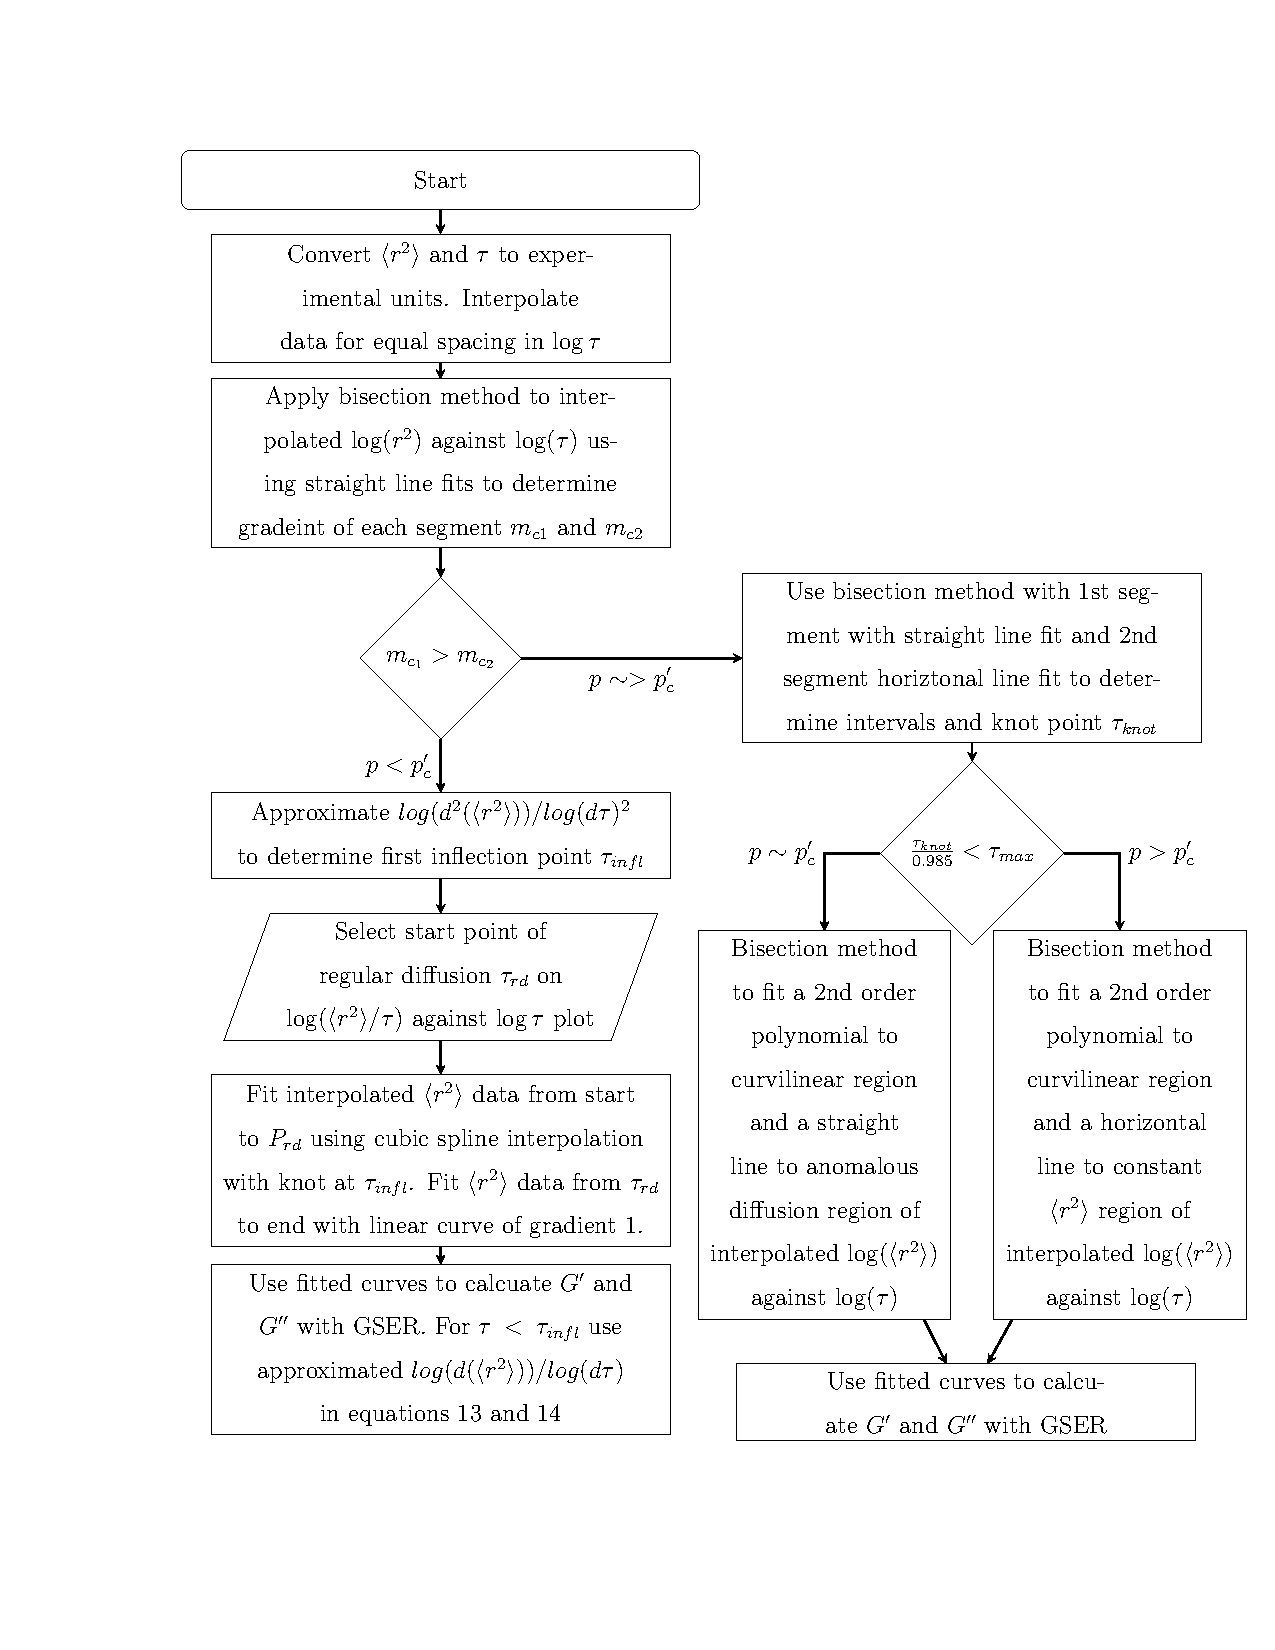
\includegraphics[width=0.7\linewidth]{FittingFlowDigram.pdf}
    \caption{Flow diagram of procedure used to determine if $p<p_c^{'}$, $p\approx p_c^{'}$' or $p>p_c^{'}$, determine curve region boundaries and fit the MSD data prior to calculation of $G^{'} (\omega)$ and $G^{''} (\omega)$}.
    \label{fig:flowchart}
\end{figure}


\textbf{Fitting procedure}
Fitting of data is a non-trivial task and prone to errors and biases. A functional form of the MSD curve is not known. In effort to apply power-law behaviour to measured MSD data often time-dependent diffusion coefficients are locally fitted to account for non-power law scaling in regions of the data. Using the GSER to interpret MSD in terms of $G^{'} (\omega)$ and $G^{''} (\omega)$ is particularly sensitive to inaccuracies in fitting due to the use of the derivative of MSD within sine and cosine terms.
In this work, knowledge of the expected form of the MSD over sub-regions of $\tau$ was used to fit the MSD data before applying the GSER. A semi-automated fitting regime was developed which determines if the MSD results from a lattice correspond to  $p<p_c^{'}$,  $p\approx p_c^{'}$ or $p>p_c^{'}$, and adjusts the fitting procedure appropriately. Initially, both the MSD and $\tau$ are converted from Monte Carlo units to experimental units (as defined in the main text in section entitled ‘calculation of $G^{'} (\omega)$ and $G^{''} (\omega)$ using equations 3 and 4 respectively). They are then interpolated using a cubic spline interpolation to reduce the number of data points to fit to $1\times10^5$ and give $\tau$ equal spacing on a log scale. A bisection technique was employed several times to determine the limits of regions identified for each case. The technique applied two-segment piecewise least squared fits of either linear or cubic functions to the data to adjoining MSD curve regions. The point of transition between regions was determined by using the bisection method to find the knot point which minimised the mean square error of the fits. A flow diagram of the fitting procedure is shown in Figure \ref{fig:flowchart}.

\end{document}